\resizebox{\textwidth}{!}{
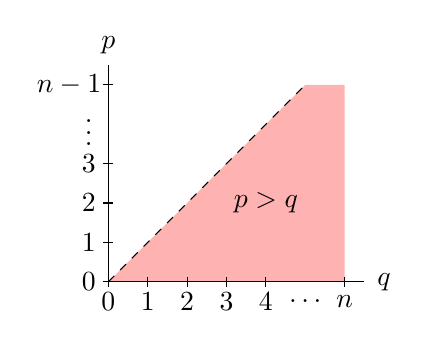
\begin{tikzpicture}[scale=.5]
%Región p > q
\filldraw[draw opacity=0, fill=red!30] (0,0) -- (5,5) -- (6,5) -- (6,0) -- cycle;
\draw[dashed] (0,0) -- (5,5);

\draw (0,5.5) -- (0,0) -- (6.5,0);
\draw (7,0) node {$q$};
\draw (0,6) node {$p$};

%q axis
\foreach \x in {0,...,4}
{
\draw (\x,-0.125) -- (\x,0.125);
\draw (\x,-0.5) node {$\x$};
}

\draw (5,-.5) node {$\dots$};

\draw (6,-0.125) -- (6,0.125);
\draw (6,-.5) node {$n$};

%p axis
\foreach \x in {0,...,3}
{
\draw (-0.125,\x) -- (0.125,\x);

\draw (-.5,\x) node {$\x$};
}

\draw (-.5,4) node {$\vdots$};

\draw (-0.125,5) -- (0.125,5);
\draw (-1,5) node {$n-1$};

\draw (4,2) node {$p > q$};
\end{tikzpicture}
}